
\textbf{Thesis Statement:} I propose a novel, neural-based mention-pair model for cross-document coreference resolution for events, which uses few lexical features and addresses shortcomings of traditional clustering approaches.  I will extend this work by jointly modelling both entities and events, while using structured information (e.g, parse trees).  Last, we aim to improve mention detection, whereby we develop an all-inclusive, end-to-end system which jointly resolves mention boundaries and coreference predictions.

\vspace{20mm}
\section{Problem Statement}
Coreference resolution is the task of identifying -- within a single text or across multiple documents -- which \textit{mentions} refer to the same underlying discourse object. 

A \textbf{mention} is a particular instance of word(s) in a document which represent an \textit{entity} or \textit{event}, such as \textit{Barack Obama}, \textit{he}, or \textit{announced}.

An \textbf{entity} may be a person, location, time, or an organization.  The mentions which refer to them may be \textit{named}, \textit{nominal}, or \textit{pronominal}:
\begin{itemize}
\item Named mentions are represented by proper names (e.g., Andr\'e Benjamin or Pakse, Laos) 
\item Pronominal mentions are represented by pronouns (e.g., she or it)
\item Nominal mentions are represented by descriptive words, not composed entirely of a named entity or pronouns (e.g., The well-spoken citizen)
\end{itemize}

An \textbf{event} can generally be thought of as a specific action.  Quine \cite{quine1985} was the first to propose that an event refers to a physical object which is grounded to a specific time and location, and that two events are identical (i.e., co-referent) if they share the same spatiotemporal location.  This definition has become the general consensus within the community.  Specifically, two co-referent events must share the same \textit{properties} and \textit{participants}.  For example, in Figure \ref{fig:corpus}, sentences \#1 and \#2 contain the co-referent events (``placed'' and ``put''), yet neither are co-referent with events in sentence \#3.  Often times, the participants (arguments) may be referred to in different ways, implied, or missing altogether.

\begin{figure}[ht]
\centering
	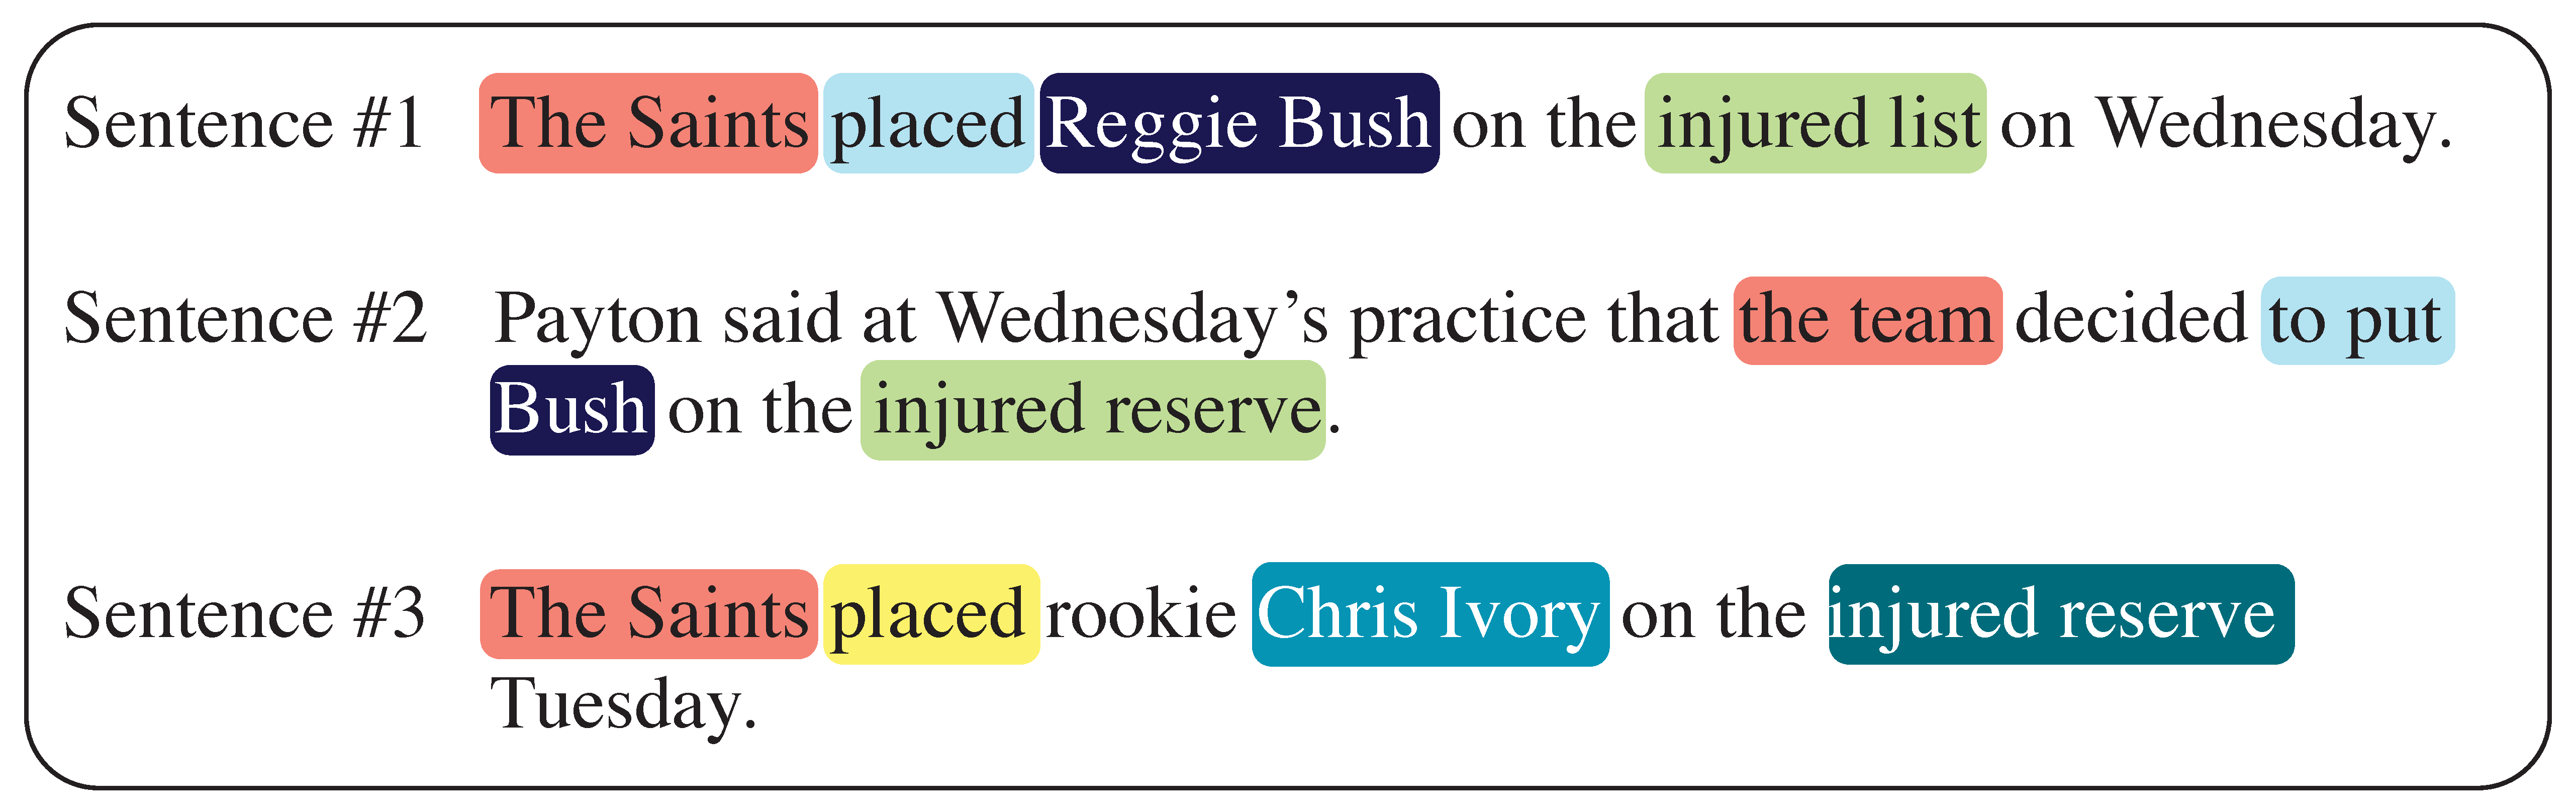
\includegraphics[width=0.65\textwidth]{graphics/corpus}
	\caption{Sample of a coreference resolution corpus (ECB+), depicting gold coref mentions as having shared box colors.}
	\label{fig:corpus}
\end{figure}

Coreference resolution is concerned with linking either entities together and/or events together; that is, entities shall not be linked to events, and doing so would be considered an incorrect link.  Although one may be interested in evaluating coreference systems by their ability to correctly link \textit{pairs} of mentions \cite{parma}, coreference resolution is ultimately a clustering task, whereby we wish to group all like-mentions together, as shown with colored boxes in Figure \ref{fig:corpus}.  Specifically, coreference systems aim to find a globally-optimal fit of mentions to clusters, whereby every mention $m$ in the corpus is assigned to exactly one cluster $C$, such that every ${m_i,m_j} \in C$ are co-referent with each other.  If a given $m_i$ is not anaphoric with any other $m_j$, then it should belong to its own $C$ with a membership of one.

Given a corpus of text documents, coreference resolution can be performed and evaluated on either a \textbf{within-document} or \textbf{cross-document} basis:

\begin{itemize}
\item \textbf{Within-document} is when each mention may only link to either (1) no other mention; or (2) other mentions which are contained in the same document.  Even if the gold truth data denotes a mention should link with a mention from a different document, we ignore these links during the evaluation.
\item \textbf{Cross-document} is when the entire corpus is available for linking; a mention is eligible to be co-referent with mentions in any other document, and the evaluation reflects the same.  As described in \cite{revisit:16}, cross-document evaluation is normally conducted by transforming the entire corpus into a ``meta-document."
\end{itemize}

\section{Coreference Systems}

\subsection{Mention Detection}
\subsection{Coreference Resolution}
\section{Motivation}



